\documentclass{beamer}
\graphicspath{ {./images/} }
\usepackage{wrapfig}
\usepackage{minted}
\usemintedstyle{monokai}

%Information to be included in the title page:
\title{PM 6 - Understanding Geometric Objects With Computer Algebra System}
\author{Adrina Esfandiari, Bowen Dai, Jessica Ni, Xena Jiang
\newline Mentor: Erica Liu}
\institute{WiM Directed Reading Program}
\date{2025}

\begin{document}

\frame{\titlepage}

\begin{frame}
\frametitle{Overview}
In this presentation, we will go over the following: 
\pause
\begin{itemize}
    \item Introduction to definitions/terminology
    \pause
    \item Important theorems and results
    \pause
    \item Application of Gröbner bases to Sudoku puzzles
    \pause
    \item Working algorithm to solve given Sudoku puzzles + live demo
\end{itemize}
\end{frame}

\begin{frame}{Full Document}
Scan here for the full document containing more detailed definitions and proofs:
\newline
\begin{figure}
    
\includegraphics[width=0.45\linewidth]{images/DRP 2025 PM 6 Full Document.png}
    \centering
\end{figure}
    
\end{frame}

\begin{frame}
\frametitle{Multi-variable Monomial and Polynomial}
\textbf{Monomial:} $$x_1^{\alpha_1} \cdot x_2^{\alpha_2} \cdots x_n^{\alpha_n}$$ for a monomial of n variables, $x_1, x_2,..., x_n$
\begin{itemize}
 \item<1-> Commonly written as $x^\alpha$
 \item<1-> $x^3y^2$ is a multivariable monomial
\end{itemize}
\leavevmode
\newline
\textbf{Polynomial:}
$$f=\sum_\alpha a_\alpha x^\alpha$$
\begin{itemize}
 \item<1-> $k[x_1,x_2,\dots,x_s]$ is the set of all polynomials with variable $x_1,x_2,\dots,x_s$
 \item<1-> $f=2x^3y^2z-3xyz + \frac{3}{2}y^3z^3 +y^2$ is a polynomial in $\mathbf{Q}[x, y, z]$
\end{itemize}\leavevmode
\end{frame}

\begin{frame}
\frametitle{Affine Variety}
We commonly write it as: 
$$\mathbf{V}(f_1, \dots, f_s)$$
Affine variety is the set of solutions in $k^n$ to a system of equations $f_1, f_2, f_3,\dots, f_s$.  
$$\mathbf{V}(f_1, \dots, f_s) = \{(a_1,\dots,a_n) \in k^n | f_i(a_1, \dots, a_n) = 0 , \forall 1 \le i \le s\}.$$

\begin{Examples}
\begin{itemize}
    \item<1-> $\mathbf{V}(x^2 + y^2 -1)$ contains all the values in $\mathbf{R}$ that makes $x^2 + y^2 -1 = 0$ true, which is all the points in the circle
    \item<1-> \textbf{$\mathbf{V}(y-x, y + x)$} contains all the values in $\mathbf{R}$ that makes $y-x = 0, y + x = 0$ true; visualized graphically, it is the intersection of two functions, which is $(0, 0)$
\end{itemize}
\end{Examples}

\end{frame}

\begin{frame}
\frametitle{Ideals}
\textbf{Ideal: $I$} the set of polynomials 
\newline
$I \subseteq{k[x_1, x_2,..., x_n]}$ 
    \begin{itemize}
        \item<1-> $0 \in I$
        \item<1-> $f, g \in I$ then $f+g \in I$
        \item<1-> If $f \in I$ and $h\in k[x_1, x_2,..., x_n]$, then $hf \in I$
    \end{itemize}
    Ideals commonly comes in the form of $\langle f_1, f_2, f_3, \dots, f_s \rangle$ where $$\langle f_1, f_2, f_3, \dots, f_s \rangle = \{\sum_{i=1}^sh_if_i|h_1,\dots h_s \in k[x_1, x_2,..., x_n]\} $$
\end{frame}

\begin{frame}
\frametitle{Ideal Examples}
\textbf{Ideal belonging problem:}
    Does $x^2-2x+2-y$ belong in $\langle x-1-t, y-1-t^2\rangle$? \pause
\newline 
\\
    Yes! $x^2-2x+2-y = (x-1+t)(x-1-t) + (-1)(y-1-t^2)$
\\ this is in the form of $$\sum_{i=1}^sh_if_i$$

\end{frame}




\begin{frame}
\frametitle{Relationship between Affine Variety and Ideals}
When we are trying to find $V(f_1, f_2, \dots,f_n)$ and $\langle f_1, f_2, \dots, f_s\rangle = \langle g_1, g_2, \dots, g_s\rangle$ 
\leavevmode
\newline

then...
\begin{itemize}
\item<1->$V( g_1, g_2, \dots, g_s) = V(f_1, f_2, \dots,f_n)$
\end{itemize}

\end{frame}


\begin{frame}{Monomial Ideal}
    Monomial ideal is a special special polynomial ideal where it can be written in the form of $$I = \langle x^{a_1}, x^{a_2}, x^{a_3} \dots\rangle$$
    \begin{itemize}
    % \item<1-> when written in this form $I = \langle x^{a_1}, x^{a_2}, x^{a_3} \dots\rangle$, the generators $x^{a_1}, x^{a_2}, x^{a_3} \dots$ is called the minimal basis of the ideal \pause
    % \item<1-> $ \forall f\in I$, $I$ is a monomial ideal, then every term of $f$ must be some monomial product of $x^{a_i}$.\pause
    % \item<1-> the minimal basis is unique and the minimal basis is finitely generated (see Dickson's lemma)
    \end{itemize}
\end{frame}


\begin{frame}{Ideal generated by leading terms of an ideal}
$$\langle LT(I)\rangle$$
\textbf{Leading term} is a term of a polynomial
\begin{itemize}
    \item<1-> Determine a monomial ordering, order the terms of the polynomial
    \item Leading term is the first term of the ordered polynomials. 
\end{itemize}
\begin{Examples}
    $f=2x^3y^2z + \frac{3}{2}y^3z^3 -3xyz +y^2$ \pause
    \newline
    $f=2x^3y^2z-3xyz + \frac{3}{2}y^3z^3 +y^2$ \pause
    \newline
    $f=$\alert{$2x^3y^2z$}$-3xyz + \frac{3}{2}y^3z^3 +y^2$ 
\end{Examples}

\end{frame}

\begin{frame}{Ideal generated by leading terms of an ideal}
    $$\langle LT(I)\rangle$$
    \begin{itemize}
    \item<1-> $LT(I)$ is the leading term of every polynomial in ideal $I$
    \item<1-> $\langle LT(I)\rangle$ is the ideal generated by those leading term
    \end{itemize}
\end{frame}

\begin{frame}{Important Theorems and Results:}
\textbf{Dickson's Lemma:} \\
 Let $I = \langle x^\alpha \mid \alpha \in A \rangle \subset k[x_1, \dots, x_n]$ be a monomial ideal. Then $I$ can be written in the form 
    \[
    I = \langle x^{\alpha(1)}, \dots, x^{\alpha(s)} \rangle,
    \]
    where $\alpha(1), \dots, \alpha(s) \in A$. In particular, $I$ has a finite basis. \\ 
    \pause
    \begin{block}{Results:}
        \begin{itemize}
        \item<1-> Necessary for the proof of Hilbert Basis theorem. 
        \item<1-> Ensures finite Gröbner basis exists. 
        
    \end{itemize}
    \end{block}   
\end{frame}

\begin{frame}{Important Theorems and Results:}
    \textbf{Hilbert Basis Theorem:} \\
    Every ideal \( I \subseteq k[x_1, \dots, x_n] \) has a finite generating set. In other words, \( I = \langle g_1, \dots, g_t \rangle \) for some \( g_1, \dots, g_t \in I \).
    \\ 
    \textit{Example:} $I = \left\langle x^2 + y^3 - z^5,\; xyz + 1,\; x^3 y^2 z^4 - 7xy + z^2,\; x^2 z - y^4,\; \dots \right\rangle$ will have a finite generating set. 
    \begin{block}{Results:}
        \begin{itemize}
            \item <1-> Any affine variety can be defined by a finite number of equations, no infinite constraints are needed. 

        \end{itemize}
    \end{block}
\end{frame}

\begin{frame}{Important Theorems and Results:} 
    \textbf{Gröbner Bases:}
        Let $I$ be an ideal from $k[x_1, \cdots x_n]$. Fix a monomial ordering. 
        A finite subset $G = \{g_1, \dots, g_r\} \subseteq I$ is called a \emph{Gröbner basis} for $I$ if:
        \[
        1. \quad I = \langle g_1, \cdots, g_r \rangle
        \]
        \[
        2. \quad \langle \text{LT}(g_1), \dots, \text{LT}(g_r) \rangle = \langle \text{LT}(f) \mid f \in I \rangle
        \]
    \textbf{Property of G:} \\
    If \( G = \{g_1, \dots, g_r\} \) is a Gröbner basis for an ideal,  then every polynomial \( f \in k[x_1, \dots, x_n] \) can be divided by \( G \), and the remainder satisfies:
    \begin{itemize}
    \item The remainder is \textbf{unique}.
    \item The remainder is \textbf{zero} if and only if \( f \in I \).
    \end{itemize}
\end{frame}

\begin{frame}{Important Theorems and Results:}
 \textbf{Results:} \\
    This helps us to solve the ideal membership problem!! \\
    \textit{Example:}
            
        Let our polynomial ring be \( \mathbb{Q}[x, y] \). Let $I =  \langle f_1, f_2 \rangle = \langle x^2 + y,\ xy - 1 \rangle$.\\
        
        \\ \textbf{Question:} Does $f = x^3y + x \in I$? \\
        
        We compute a Gröbner basis using lexicographic order with \( x > y \). Then $G = \{ y^2 + x,\  xy - 1, \ x^2 + y \}$. By performing multivariate polynomial division of $f$ with respect to $G$, the remainder is 0 hence, \( f \in I \). 
    
\end{frame}



% sudoku application begins here
\begin{frame}{Sudoku Application: Rules}
To begin, we will consider a 4x4 sudoku grid with the following rules:
\begin{wrapfigure}{l}{0.35\textwidth} 
    \centering
    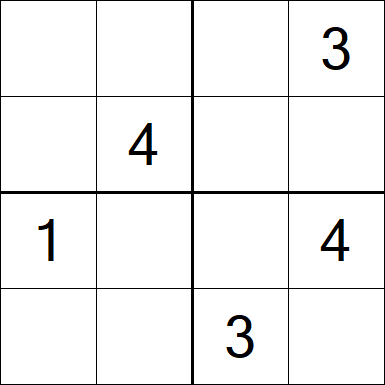
\includegraphics[width=0.35\textwidth]{images/1.png}
\end{wrapfigure}
\pause
\begin{enumerate}
    \item All values must be integers between 1 and 4 \pause
    \item The sum of every row, column, and 2x2 block must be 10 \pause
    \item No two blocks in the same row, column, or 2x2 block can be equal
\end{enumerate}
\end{frame}

\begin{frame}{Sudoku Application Overview}
Now, using what we have learned, we can find a solution to any proper 4x4 sudoku with the following steps:
\pause
    \begin{itemize}
        \item Assign the variables $x_0, x_1, ... , x_{14}, x_{15}$ to each grid \pause
        \item Create polynomials representing each rule from before \pause
        \item Generate an ideal using these polynomials \pause
        \item Use an algorithm (Buchberger's algorithm) to generate Gröbner basis \pause
        \item Find the variety (solutions) of the ideal using generated basis
    \end{itemize}
\end{frame}
\begin{frame}{Polynomials Needed}
For $0 \leq i, j\leq 15$, consider the following polynomials used to generate our ideal:
\newline
\pause
    \begin{itemize}
    
        \item $F(x_i) = (x_i-1)(x_i-2)(x_i-3)(x_i-4)$
        \newline 
        \pause
        \item $G(x_i, x_j) = \frac{F(x_i)-F(x_j)}{x_i - x_j}$
        \newline
        \pause
        \item $x_i - a$ for $1\leq a \leq 4$ (the pre-existing squares)
    \end{itemize}
\end{frame}

\begin{frame}{Ideal and Gröbner Basis Generated}
    Now, we can create an ideal $I$ using these polynomials and use Buchberger's algorithm to generate the unique Gröbner basis G with the following properties: \pause
    \begin{itemize}
        \item If the sudoku is proper, each element of this basis is of the form $x_i - a_i $ for $1\leq a_i\leq4$
        \pause
        \item The solutions to the variety of $I$ is simply the solution to setting each element of $G$ to zero
        \pause
        \item Thus, each $a_i$ describes the value present in grid $x_i$ (or the solution to the sudoku) since each $x_i = a_i$
    \end{itemize}
\end{frame}
\begin{frame}[fragile]
\frametitle{Implementation}
    \begin{minted}
    [
    bgcolor = black,
    fontsize = \footnotesize,
    linenos
    ]{python}
    import itertools
    
    #initialize varibles x_0,...,x_15
    var_names = ['x_{}'.format(i) for i in range(0,16)]
    
    #initialize polynomial ring with x_0,...,x_15
    R = PolynomialRing(QQ, var_names, order='lex')
    R.inject_variables()

    #generate the polynomial (x_i-1)(x_i-2)(x_i-3)(x_i-4) 
    #These polynomials restrict that x_i must equals to 
    #1, 2, 3, or 4
    poly_List = []
    for x in R.gens(): 
        poly_List.appen(prod([(x-i) for i in [1..4]]))
    \end{minted}
\end{frame}

\begin{frame}[fragile]
\frametitle{Implementation}
    \begin{minted}
    [
    bgcolor = black,
    fontsize = \footnotesize,
    linenos,
    firstnumber = last
    ]{python}
    row_List = [] #generate a list of polynomial for each row
    for i in range(4):
        temp =[]
        for j in range(4):
            temp.append(poly_List[i*4+j])
        row_List.append(temp)
    
    col_List = [] #generate a list of polynomial for each column
    for i in range(4):
        temp = []
        for j in range(4):
            temp.append(poly_List[i+4*j])
        col_List.append(temp)
    
    block_List =[] #generate a list of polynomial for each block
    for i in range(4):
        start = (i//2)*8 +(i%2)*2
        temp = []
        for j in range(4):
            temp.append(poly_List[start + j%2 + (j//2)*4])
        block_List.append(temp)
    \end{minted}
\end{frame}

\begin{frame}[fragile]
\frametitle{Implementation}
    \begin{minted}
    [
    bgcolor = black,
    fontsize = \footnotesize,
    linenos,
    firstnumber = last
    ]{python}
    # combine all lists 
    adjacent_List = row_List + col_List + block_List
    diff_List = []
    for l in adjacent_List:
        comb = list(itertools.combinations(l,2))
        # take all possible combinations and eliminate the 
        # factor (x_i-x_j), so x_i =\= x_j if they are in
        # the same row, column or block
        for c in comb: 
            diff = c[0] - c[1]
            vars = diff.variables()
            diff_List.append(diff/(vars[0]-vars[1]))

    #clues from sudoku
    initial_clues = [x_3-3,x_5-4,x_8-1,x_11-4,x_14-3]

    #generate the ideal using the clues, non-repetitive 
    #restrictions and number restriction of each variables
    I = R.ideal(initial_clues + diff_List + poly_List)
    G = I.groebner_basis()
    show(G)
    \end{minted}
\end{frame}
\begin{frame}[fragile]
\frametitle{Result}
\begin{minted}
    [
    bgcolor = black,
    fontsize = \footnotesize
    ]{python}
    # the groebner basis of the ideal I is the solution of 
    # the sukodu
    [x_0 - 2, x_1 - 1, x_2 - 4, x_3 - 3, 
     x_4 - 3, x_5 - 4, x_6 - 1, x_7 - 2, 
     x_8 - 1, x_9 - 3, x_10 - 2, x_11 - 4, 
     x_12 - 4, x_13 - 2, x_14 - 3, x_15 - 1]
\end{minted}
    
\end{frame}

\begin{frame}{Conclusion and Further Applications}
    Today, we went over:
    \pause
    \begin{itemize}
        \item Varieties, ideals, and Gröbner bases
        \pause
        \item Dickson's Lemma and Hilbert Basis Theorem
    w    \pause
        \item Application to solving sudoku puzzles in computer algebra systems
        \pause
    \end{itemize}
    Further applications: \pause
    \begin{itemize}
        \item Similar usage of Gröbner bases to solve other games (eg. minesweeper) or more complex sudoku puzzles (eg. 9x9)
        \pause
        \item Algebraic Geometry appears in other areas of pure math such as topology, complex analysis, number theory and more. %sorry i'm not sure what specifically we wanted to talk about here
        % dw, I have a suggestion: Gröbner bases can also be used to solve intersections of subvarities by eliminating variables. It is an important techniques in elimination theory.
    \end{itemize}
\end{frame}
\end{document}